\documentclass[letterpaper]{article}

\usepackage[in,plain]{fullpage}

\usepackage{algorithm}
\usepackage{algorithmic}
\usepackage{amsmath}
\usepackage{amssymb}
\usepackage{graphicx}

\usepackage{subfigure}

\usepackage{hyperref}
\usepackage{url}

\linespread{1.3}

\let\oldthebibliography=\thebibliography
\let\endoldthebibliography=\endthebibliography
\renewenvironment{thebibliography}[1]{%
  \begin{oldthebibliography}{#1}%
    \setlength{\parskip}{0ex}%
    \setlength{\itemsep}{0ex}%
}%
{%
  \end{oldthebibliography}%
}

\begin{document}

\title{\vspace{-40pt} Notes}

\author{}
\date{}

\maketitle

\vspace{-20pt}
\noindent{\bf{\large Related Work}}: 

Greytak \cite{Greytak09} provides a detailed treatment of how to evaluate the probability of success for a point robot under motion uncertainty by considering truncated Gaussians but does not consider sensing uncertainty or a feedback law for dealing with the uncertainty. Toussaint \cite{Toussaint09b} truncates the Gaussian belief to compute a revised distribution over the state in the context of approximate inference control (which provides a solution to the stochastic optimal control problem) but does not explicitly compute the probability of success. Erez and Smart \cite{Erez10} use the approach suggested in \cite{Toussaint09b} to approximate the Gaussian belief (represented as a Gaussian mixture) along one active constraint and solve the stochastic optimal control problem using differential dynamic programming (DDP) in belief space. Their method does not easily generalize to multiple constraints. Vitus and Tomlin \cite{Vitus11} use Boole's inequality to compute a conservative bound for the probability of success to solve a chance constrained optimal control problem. They do not truncate the beliefs while processing constraints, thereby obtaining a very conservative estimate of the actual probability of success.

There is also a considerable body of work on Kalman filtering with state constraints. \cite{Simon09} outlines several methods to perform state estimation under (linear and nonlinear) equality and inequality state constraints, one of which is to truncate Gaussian densities along the specified constraints.

\vspace{10pt}
\noindent{\bf{\large Truncated Gaussians}}: 

Given a $n$-dimensional Gaussian belief $\mathcal{N}[\mathbf{x}|\hat{\mathbf{x}}, \Sigma]$ and a (locally-)convex feasible region $\mathcal{X}_{free}^{C}$ bound by $m$ hyperplanes $\{\mathbf{a}_{i}^T \mathbf{x} - b_{i} = 0\}$: $\mathcal{X}_{free}^{C} \equiv \bigcap \limits_{i = 1}^{m} {\{\mathbf{a}_{i}^T \mathbf{x} > b_{i}\}}$, we want to estimate the truncated Gaussian $\mathcal{N}[\mathbf{x}|\underline{\hat{\mathbf{x}}}, \underline{\Sigma}]$ that best approximates the Gaussian distribution of the samples drawn from $\mathcal{N}[\mathbf{x}|\hat{\mathbf{x}}, \Sigma]$ that lie in $\mathcal{X}_{free}^{C}$.

We propose to construct the truncated Gaussian $\mathcal{N}[\mathbf{x}|\underline{\hat{\mathbf{x}}}, \underline{\Sigma}]$ by sequentially truncating the original Gaussian $\mathcal{N}[\mathbf{x}|\hat{\mathbf{x}}, \Sigma]$ along each of the $m$ half-space constraints: $\{\mathbf{a}_{i}^T \mathbf{x} > b_{i}\}, i = 1\ldots,m$, where $\mathbf{a}_i$ is the $i^{\mathrm{th}}$ hyperplane normal and $b_i$ is the offset. Let $\mathcal{N}[\mathbf{x}|\hat{\mathbf{x}}_{i-1}, \Sigma_{i-1}]$ be the Gaussian obtained after sequentially truncating $\mathcal{N}[\mathbf{x}|\hat{\mathbf{x}}, \Sigma]$ along $(i-1)$ constraints.

Following the derivation of \cite{Toussaint09a}, we process the $i^{\mathrm{th}}$ constraint by first transforming the problem such that the Gaussian $\mathcal{N}[\mathbf{x}|\hat{\mathbf{x}}_{i-1}, \Sigma_{i-1}]$ becomes a standard Gaussian and the constraint is aligned along a reference unit vector $\mathbf{e} = (1,0,\ldots,0)$. If $\Sigma_{i-1} = C^TC$ be the Cholesky decomposition $(\Sigma_{i-1}^{-1} = C^{-1}C^{-T})$, we can express the Gaussian $\mathcal{N}[\mathbf{x}|\hat{\mathbf{x}}_{i-1}, \Sigma_{i-1}]$ in the coordinate system of $\mathbf{y} = C^{-T}(\mathbf{x} - \hat{\mathbf{x}}_{i-1})$ as:
\begin{equation*}
\mathcal{N}[\mathbf{x}|\hat{\mathbf{x}}_{i-1}, \Sigma_{i-1}] \propto \mathrm{exp}\{-\frac{1}{2}(\mathbf{x} - \hat{\mathbf{x}}_{i-1})^{T} \Sigma^{-1} (\mathbf{x} - \hat{\mathbf{x}}_{i-1})\} \longrightarrow \mathrm{exp}\{-\frac{1}{2}\mathbf{y}^T\mathbf{y}\} \equiv \mathcal{N}[\mathbf{y}|\mathbf{0},I]
\end{equation*}
where $\mathcal{N}[\mathbf{y}|\mathbf{0},I]$ is a Gaussian with zero mean and unit variance. By substituting $\mathbf{x} = (C^T\mathbf{y} + \hat{\mathbf{x}}_{i-1})$, the constraint $\{\mathbf{a}_{i}^T \mathbf{x} > b_{i}\}$ is transformed to $\{\mathbf{u}_{i}^T \mathbf{y} > v_{i}\}$, where $\mathbf{u}_i = C\mathbf{a}_i/|C\mathbf{a}_i|$ is a normalized vector and $\mathbf{v}_i = (b_i - \mathbf{a}_i^T\hat{\mathbf{x}}_{i-1})/|C\mathbf{a}_i|$.

We compute a rotation matrix $R$ that rotates the reference unit vector $\mathbf{e} = (1,0,\ldots,0)$ onto the normalized vector $\mathbf{u}_i$ i.e. $\mathbf{u}_i = R\mathbf{e}$. The Gaussian $\mathcal{N}[\mathbf{y}|\mathbf{0},I]$ and the constraint are transformed in a rotated coordinate system $\mathbf{y}' = R^{-1}\mathbf{y}$ as $\mathcal{N}[\mathbf{y'}|\mathbf{0},I]$ and $\{(R^{-1}\mathbf{u}_i)^T\mathbf{y'} > v_{i}\} \equiv \{\mathbf{e}^T\mathbf{y'} > v_{i}\}$ respectively. The problem is now transformed to a simplified 1D form where the standard Gaussian distribution $\mathcal{N}[\mathbf{y'}|\mathbf{0},I]$ is truncated along the first axis in the $\mathbf{y}'$ coordinate system.

The mean and variance of a standard Gaussian distribution $\mathcal{N}[v|0,1]$ truncated along a linear constraint $v \geq v_i$ are given by $\mu = (e^{-v_i^2/2}/n)$ and $\sigma^2 = (1 + v_i\mu - \mu^2)$ respectively, where $n = \sqrt{\pi/2}(1 - \mathrm{erf}(v_i/\sqrt{2}))$ \cite{Toussaint09a}. Given the mean $\mu$ and variance $\sigma^2$ of the $v_i$-truncated standard Gaussian, the truncated standard Gaussian in the $\mathbf{y}'$ coordinate system is obtained as $\mathcal{N}[\mathbf{y'}|(\mu,0,\ldots,0)^T, \mathrm{diag}(\sigma^2,1,\ldots,1)]$. The mean and variance of the $i^{\mathrm{th}}$ truncated Gaussian $\mathcal{N}[\mathbf{x}|\hat{\mathbf{x}}_{i}, \Sigma_{i}]$ are then obtained by applying the reverse transform $\mathbf{x} = C^{T}R\mathbf{y'} + \hat{\mathbf{x}}_{i-1}$:
\begin{align*}
\hat{\mathbf{x}}_{i} &= C^TR\cdot(\mu,0,\ldots,0)^T + \hat{\mathbf{x}}_{i-1} \\
\Sigma_{i} &= C^TR\cdot\mathrm{diag}(\sigma^2,1,\ldots,1)\cdot R^TC
\end{align*}

We obtain the desired truncated Gaussian $\mathcal{N}[\mathbf{x}|\underline{\hat{\mathbf{x}}}, \underline{\Sigma}]$ by sequentially processing the $m$ half-space constraints i.e. $\underline{\hat{\mathbf{x}}} = \hat{\mathbf{x}}_{m}$ and $\underline{\Sigma} = \Sigma_{m}$. Our experiments indicate that the order in which the constraints are processed is important but the differences in the obtained means and variances are minimal when compared to the truncated Gaussians computed using dense sampling (Fig. \ref{fig:trunc1}).

\vspace{10pt}
\noindent{\bf{\large Analytical Computation of Probability of Success}}:

Given a $n$-dimensional Gaussian belief $\mathcal{N}[\mathbf{x}|\hat{\mathbf{x}}, \Sigma]$ and a (locally-)convex feasible region $\mathcal{X}_{free}^{C}$ bound by $m$ hyperplanes $\{\mathbf{a}_{i}^T \mathbf{x} - b_{i} = 0\}$: $\mathcal{X}_{free}^{C} \equiv \bigcap \limits_{i = 1}^{m} {\{\mathbf{a}_{i}^T \mathbf{x} > b_{i}\}}$, we want to estimate the probability of success: $p(\mathbf{x} \in \mathcal{X}_{free}^{C}), \mathbf{x} \sim \mathcal{N}[\mathbf{x}|\hat{\mathbf{x}}, \Sigma]$. Exact computation of this probability requires the integration of a multivariate Gaussian distribution over the feasible region, which does not have an analytic solution. A na\"{\i}ve solution involves densely sampling the Gaussian $\mathcal{N}[\mathbf{x}|\hat{\mathbf{x}}, \Sigma]$ and counting the number of successful samples that lie in $\mathcal{X}_{free}^{C}$ to estimate the probability. This strategy is computationally expensive. We outline a method below to estimate this probability analytically.

{\bf{Method 1}}: Boole's inequality states that for a countable set of events $E_1, E_2, \ldots$, the probability that at least one of the events happens is no larger than the sum of the individual probabilities i.e. $p(\bigcup E_i) \leq \sum p(E_i)$. By using Boole's inequality, the probability $p(\mathbf{x} \in \mathcal{X}_{free}^{C})$ can be conservatively estimated as \cite{Vitus11}:
\begin{align*}
p(\mathbf{x} \in \mathcal{X}_{free}^{C}) &= 1 - p(\mathbf{x} \not \in \mathcal{X}_{free}^{C})\\
&\geq 1 - \sum\limits_{i=1}^{m}p(\mathbf{a}_{i}^T \mathbf{x} \leq b_{i})
\end{align*}
The probability $p(\mathbf{a}_{i}^T \mathbf{x} \leq b_i), \mathbf{x} \sim \mathcal{N}[\mathbf{x}|\hat{\mathbf{x}}, \Sigma]$ along the $i^\mathrm{th}$ half-space constraint is evaluated as:
\begin{align*}
p(\mathbf{a}_{i}^T \mathbf{x} \leq b_i) &= 
\frac{1}{\sqrt{2 \pi \mathbf{a}_i^T \Sigma \mathbf{a}_i}} \int_{-\infty}^{b_i} \mathrm{exp}(-\frac{(y - \mathbf{a}_i^T\hat{\mathbf{x}})^2}{2\mathbf{a}_i^T\Sigma\mathbf{a}_i})dy, ~~~ \mathrm{where} ~~ y = \mathbf{a}_i^T\mathbf{x}\\
&=\frac{1}{\sqrt{2 \pi}} \int_{-\infty}^{\frac{b_i - \mathbf{a}_i^T\hat{\mathbf{x}}}{\sqrt{\mathbf{a}_i^T\Sigma\mathbf{a}_i}}}\mathrm{exp}(-\frac{z^{2}}{2})dz\\
&=\mathrm{cdf}(\frac{b_i - \mathbf{a}_i^T\hat{\mathbf{x}}}{\sqrt{\mathbf{a}_i^T\Sigma\mathbf{a}_i}})
\end{align*}
where cdf is the Gaussian cumulative distribution function and is related to the error function erf as $\mathrm{cdf}(z) = \frac{1}{2}(1 + \mathrm{erf}(\frac{z}{\sqrt{2}}))$, which in turn can be efficiently evaluated using a series approximation. The probability estimate computed using this method can be very conservative (Figs. \ref{fig:panel1} and \ref{fig:panel2}).

{\bf{Method 2}}: Another approach is to sequentially truncate the Gaussian $\mathcal{N}[\mathbf{x}|\hat{\mathbf{x}}, \Sigma]$ along each of the $m$ half-space constraints $\{\mathbf{a}_{i}^T \mathbf{x} > b_{i}\}$ and compute the probability $p(\mathbf{x} \in \mathcal{X}_{free}^{C})$ as:
\begin{align*}
p(\mathbf{x} \in \mathcal{X}_{free}^{C}) &= 1 - p(\mathbf{x} \not \in \mathcal{X}_{free}^{C})\\
&\approx \prod\limits_{i=1}^{m}(1 - p(\mathbf{a}_{i}^T \mathbf{x} \leq b_{i}))
\end{align*}
where $p(\mathbf{a}_{i}^T \mathbf{x} \leq b_{i})$ is computed at each step using the truncated Gaussian approximation $\mathcal{N}[\mathbf{x}|\hat{\mathbf{x}}_{i}, \Sigma_{i}]$ obtained after processing the $i^{\mathrm{th}}$ constraint, as:
\begin{equation*}
p(\mathbf{a}_{i}^T \mathbf{x} \leq b_{i})=\mathrm{cdf}(\frac{b_i - \mathbf{a}_i^T\hat{\mathbf{x}}_{i}}{\sqrt{\mathbf{a}_i^T\Sigma_i\mathbf{a}_i}})
\end{equation*}

Since this method estimates the probability of success based on successive truncated Gaussian approximations, the order in which the truncated Gaussians are computed is important. In our experiments, we process the constraints in a random order and our experiments indicate that the probability of success computed using this method provides a good, though conservative, estimate of the actual probability (verified using dense sampling) and performs better than the first method (Figs. \ref{fig:panel1} and \ref{fig:panel2}). We still need to verify if the estimate is always conservative.

\vspace{10pt}
\noindent{\bf{\large To Do}}: 

\begin{itemize}
\item {\bf{Local convexification}}: We could follow the construction outlined in \cite{Comba03} to automatically decompose the workspace into locally-convex regions of free space using BSP trees. This approach generalizes to both 2D and 3D workspaces. Should the convex decomposition be static (determined in a pre-processing step) or should it be computed on the fly?
\item {\bf{Propagate truncated beliefs}}: We need to propagate the truncated beliefs at each time-step according to the dynamics and observation models while accounting for feedback (similar to LQG-MP). This could also be incorporated in an ILQG framework for local optimization of trajectories in belief space. How do we handle the fact that the mean of the posterior distribution deviates from the path and how can the probability of success be computed a priori to execution?
\item {\bf{Order of constraints}}: The method seems to depend on the order in which the constraints are processed. Is there a way to achieve order independence?
\item {\bf{Sampling time}}: The probability of success computation also depends on the sampling time duration. Since we are dealing with a discrete dynamics and observation model, this is not an issue but would be if we are dealing with continuous process models.
\item {\bf{Non-point robots}}: How can we generalize this method to handle non-point robots? Instead of considering a spherical cover for the non-point robot (oversimplified), maybe we could consider a tight fitting ellipsoid cover for the robot and use Gaussian convolution operations to obtain a better estimate of the probability of success?
\end{itemize}

\linespread{1.0}
\begin{figure}[t]
\begin{center}
\subfigure[\label{fig:trunc1}]{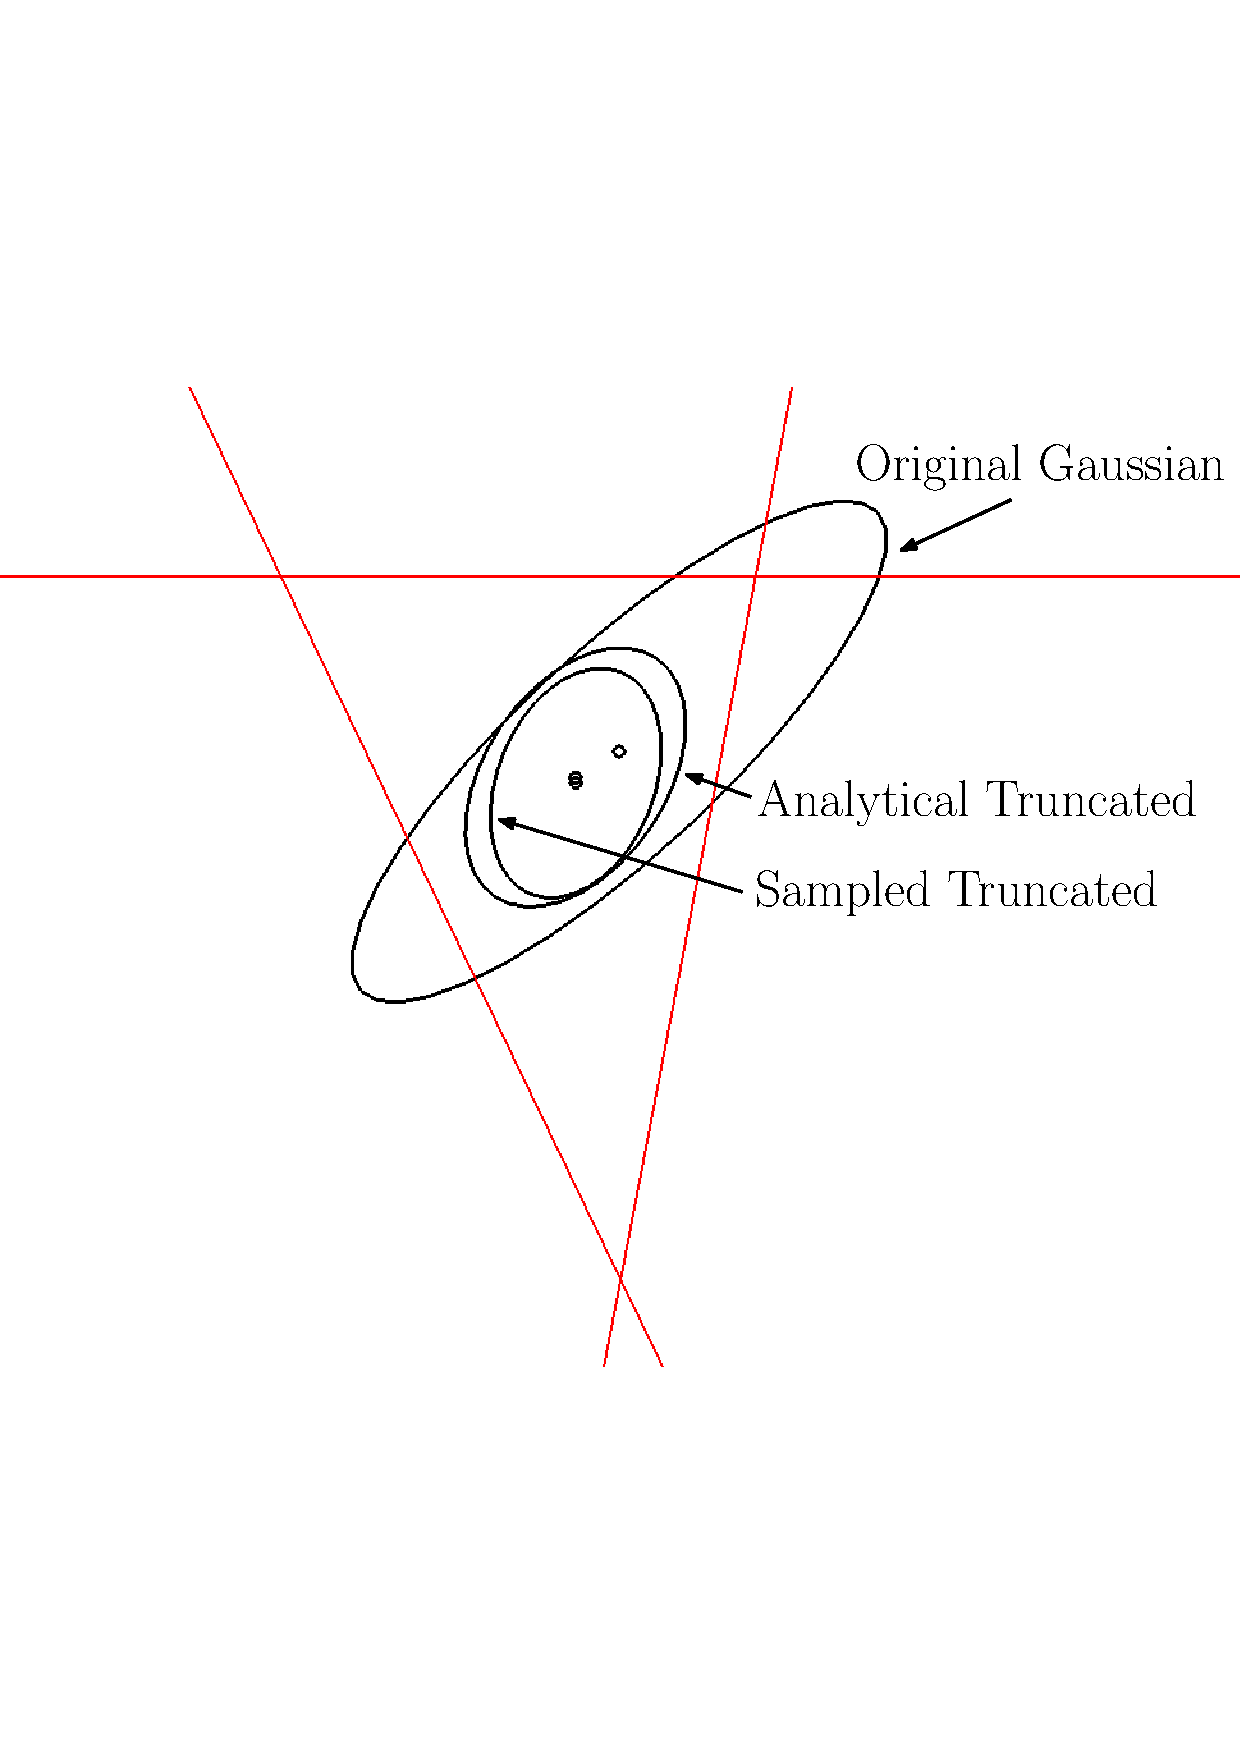
\includegraphics[trim=0mm 0mm 0mm 0mm, clip, width=0.49\linewidth]{figures/trunc1.pdf}}
\hspace{10pt}
\subfigure[\label{fig:trunc2}]{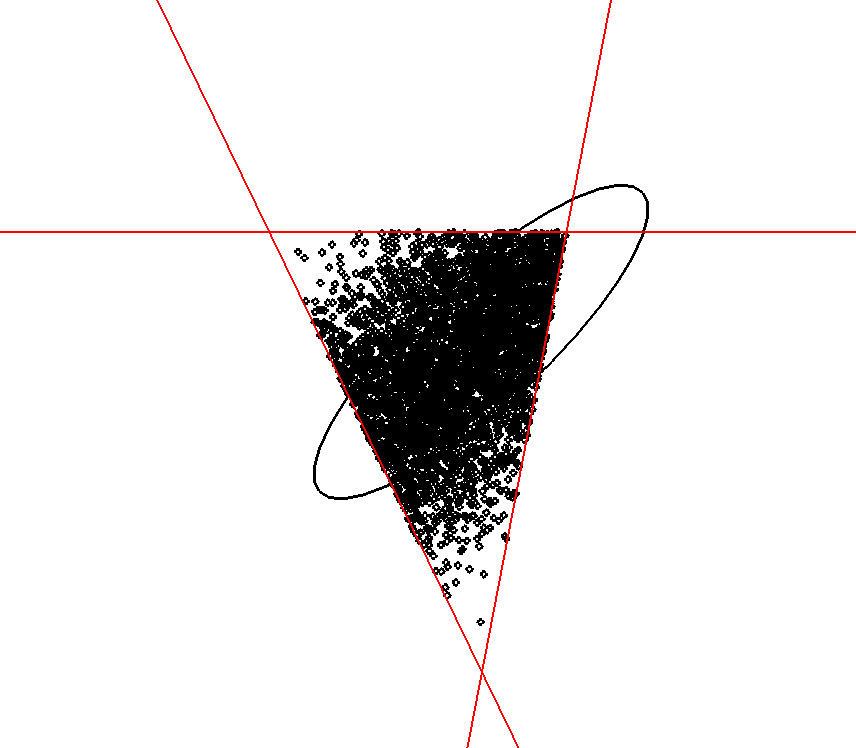
\includegraphics[trim=30mm 10mm 40mm 20mm, clip, width=0.42\linewidth]{figures/trunc2.png}}\\
\end{center}
\caption{2D Gaussian truncated by 3 half-space constraints. (a) The analytically computed truncated Gaussian is a good approximation of the sampled truncated Gaussian computed using $10000$ samples (shown in (b)). The probability of success using (i) Boole's inequality: $0.182$, (ii) Method 2: $0.341$, and (iii) Sampling: $0.369$. The result obtained using Boole's inequality is overly conservative.}
\label{fig:panel1}
\end{figure}

\begin{figure}[!bt]
\begin{center}
\subfigure[\label{fig:trunc3}]{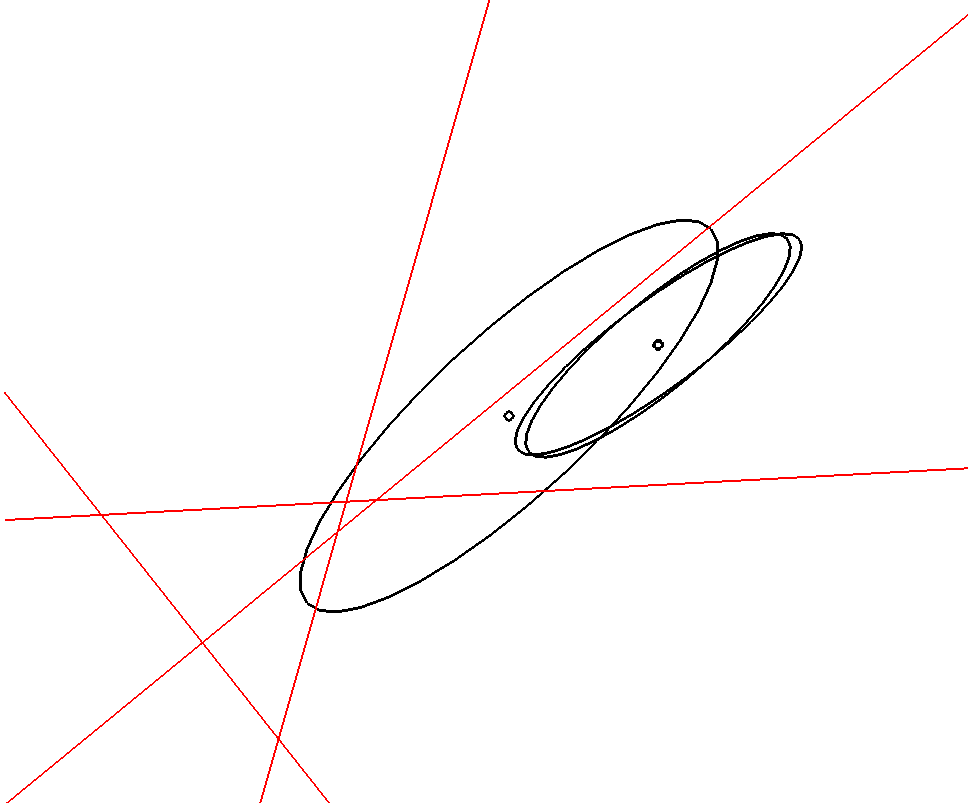
\includegraphics[trim=30mm 10mm 30mm 20mm, clip, width=0.45\linewidth]{figures/trunc3.png}}
\hspace{10pt}
\subfigure[\label{fig:trunc4}]{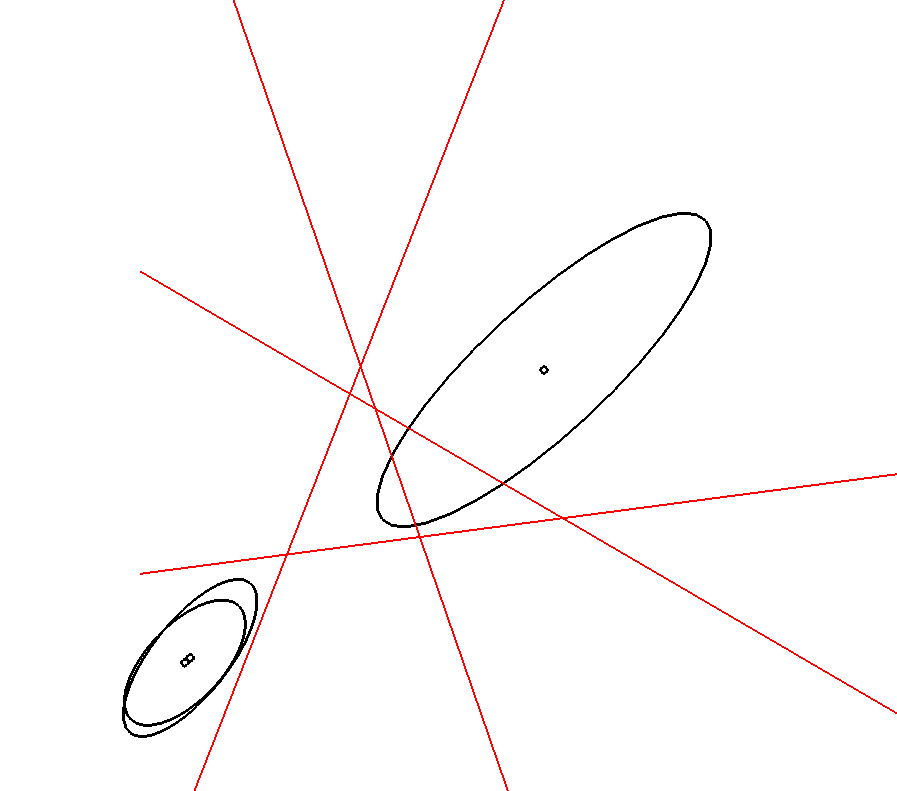
\includegraphics[trim=30mm 10mm 40mm 20mm, clip, width=0.45\linewidth]{figures/trunc4.png}}\\
\end{center}
\caption{2D Gaussian truncated by 4 randomly generated half-space constraints. (a) The probability of success using (i) Boole's inequality: $0 (-0.03)$, (ii) Method 2: $0.326$, and (iii) Sampling: $0.33$. (b) The probability of success using (i) Boole's inequality: $0 (-2.3)$, (ii) Method 2: $0.0339$, and (iii) Sampling: $0.0341$. The result obtained using Boole's inequality predicts a zero probability of success, which is not the case.}
\label{fig:panel2}
\vspace{-10pt}
\end{figure}

\begin{thebibliography}{99.}
\bibitem{Comba03} J. Comba, C. Silva. Automatic Convexification of Space Using BSP trees. \emph{Unpublished manuscript}, 2003. \url{http://www.sci.utah.edu/~csilva/papers/bsp-fill.pdf}.

\bibitem{Erez10} T. Erez, W. D. Smart. A Scalable Method for Solving High-Dimensional Continuous POMDPs Using Local Approximation. \emph{Conf. on Uncertainty in Artificial Intelligence (UAI)}, 2010. \url{http://research.engineering.wustl.edu/~etom/uai10.pdf}
    
\bibitem{Greytak09} M. Greytak. Integrated Motion Planning and Model Learning for Mobile Robots with Application to Marine Vehicles. \emph{PhD Thesis}. MIT. 2009. \url{http://web.mit.edu/hovergroup/pub/Thesis_mgreytak.pdf}

\bibitem{Simon09} D. Simon. Kalman Filtering with State Constraints: A Survey of Linear and Nonlinear Algorithms. \emph{IET Control Theory and Applications}, 2009. \url{http://academic.csuohio.edu/simond/ConstrKF/ConstrKF.pdf}

\bibitem{Toussaint09a} M. Toussaint. Technical Note: Computing moments of a truncated {G}aussian for {EP} in high dimensions. 2009. \url{http://userpage.fu-berlin.de/~mtoussai/notes/truncatedGaussian.pdf}.

\bibitem{Toussaint09b} M. Toussaint. Pros and Cons of truncated {G}aussian {EP} in the context of {A}pproximate {I}nference {C}ontrol. \emph{NIPS Workshop on Probabilistic Approaches for Robotics and Control}, 2009. \url{http://userpage.fu-berlin.de/mtoussai/publications/09-toussaint-NIPSworkshop.pdf}.

\bibitem{Vitus11} M. P. Vitus, C. J. Tomlin. Closed-loop Belief Space Planning for Linear, Gaussian Systems. \emph{IEEE Int. Conf. on Robotics and Automation}, 2011. \url{http://www.stanford.edu/~vitus/pubs/VT_IFAC_11.pdf}

\end{thebibliography}

\end{document} 